\documentclass[11pt,letterpaper]{article}
\usepackage{graphicx}
\usepackage{geometry}
\usepackage{amsmath}
\usepackage{amssymb}
\usepackage{url}
\usepackage{hyperref}
\usepackage{natbib}
\usepackage{booktabs}
\usepackage{xcolor}
\usepackage{listings}
\usepackage{microtype}
\usepackage{times}

\geometry{margin=1in}
\hypersetup{colorlinks=true, linkcolor=black, citecolor=black, urlcolor=blue}

\title{\textbf{Diagnosing the Formula: Locality-Gated, Spectrum-Based Semantic Fault Localization for Compositional NL-to-FOL Translation}}

\author{
  Anonymous Author(s)\\
  \texttt{anonymous@example.com}
}

\date{}

\begin{document}

\maketitle

\begin{abstract}
Large language models (LLMs) mistranslate compositional natural-language sentences into first-order logic (FOL), yet no existing neuro-symbolic pipeline can pinpoint which sub-component—a wrong predicate binding, a flipped quantifier, a mis-nested scope—is faulty without gold-standard annotations. We import spectrum-based fault localization (SBFL) from software engineering to address this gap, but crucially make error locality a first-class, empirically measured precondition rather than a silent assumption. A Phase-0 locality pilot on 120 FOLIO sentences reveals that only 28.9\% of wrong formulas are local ($\leq$2 faulty components), failing the pre-registered 70\% gate and constituting a primary publishable finding: compositional FOL translation errors are predominantly diffuse. Nonetheless, on the 33-sentence local subset, Ochiai-based SBFL achieves 96.8\% top-1 component-localization accuracy versus 39.2\% for random baseline, with wasted effort of 0.008 versus 0.5—confirming that the software-engineering transfer succeeds exactly when, and only when, locality holds. A mixed prover/non-prover probe bank (Z3 bounded model checking at domain size $\leq$8 plus four deterministic analytical probes) achieves a 98.9\% probe-verdict rate, supplying sufficient statistical power for Ochiai ranking. Alignment accuracy reaches 100\% via translation-time span-tagged code-style generation. Ablations show robustness across probe counts ($k$=5,10,20) and alignment-noise levels up to 20\%. We report break-even thresholds and characterize the diffuse-error regime as the dominant barrier to SBFL transfer in FOL, providing an actionable agenda for future work on targeted compositional repair.
\end{abstract}

% ─────────────────────────────────────────────────────────────────────────────
\section{Introduction}
% ─────────────────────────────────────────────────────────────────────────────

Neuro-symbolic pipelines for automated reasoning—LINC \citep{Olausson2023}, Logic-LM \citep{Pan2023}, CLOVER \citep{Ryu2025}, Code4Logic \citep{Liu2025}—share a common architecture: an LLM translates a natural-language (NL) sentence into first-order logic (FOL), a symbolic solver reasons over the result. These systems have demonstrated strong performance on structured reasoning benchmarks, yet they converge on the same bottleneck: when an LLM's FOL translation is semantically wrong, the system cannot say \emph{which part} is wrong. As Logic-LM's authors state plainly, ``no feedback is provided during regeneration because pinpointing semantic errors in translation is challenging'' \citep{Pan2023}.

The practical cost of this blind spot is high. A formula with a flipped quantifier, a dropped negation, or a mis-nested scope can silently corrupt an entire downstream reasoning chain. The field's current responses are coarse: majority voting (LINC \citep{Olausson2023}) aggregates whole-formula outputs, discarding information about \emph{where} candidates disagree; self-refinement (Logic-LM \citep{Pan2023}) reacts only to solver \emph{syntax} errors; compositional decomposition (CLOVER \citep{Ryu2025}) selects among whole-formula candidates by equivalence but never produces a per-component error signal; FoVer \citep{Pei2025} verifies a formula against a prover but does not localize within it.

Software engineering solved an analogous problem decades ago. Given a suite of tests with pass/fail outcomes and a record of which program elements each test exercised, \emph{spectrum-based fault localization} (SBFL)—Tarantula \citep{Jones2005}, Ochiai \citep{Abreu2007}, DStar \citep{Wong2014}—ranks the buggy statement by correlating element-involvement with test failures. NL$\to$FOL translation has every structural ingredient SBFL needs: the candidate formula is the ``program,'' its atomic predicate/quantifier/connective sub-components are the ``statements,'' oracle-free metamorphic probes are the ``tests,'' and a sound prover deciding a relation that holds by construction provides the ``pass/fail oracle.'' Yet this framing has never been applied to the FOL setting.

The transfer is not straightforward, however. SBFL is known to degrade with small test suites and when faults sit in ``hot'' components exercised by nearly every test \citep{Jones2005,Abreu2007}. Importing it blindly into NL$\to$FOL would be naive. The central question is therefore: \emph{under what measurable conditions does SBFL succeed at localizing compositional FOL translation errors?} We identify three governing quantities—error locality, alignment accuracy, and probe-verdict rate—and make each a first-class, empirically measured variable rather than an unstated assumption.

Our approach proceeds in six phases%
\footnote{Code: \url{https://github.com/AMGrobelnik/ai-invention-e70e3d-diagnosing-the-formula-locality-gated-sp/tree/main/round-1/experiment-1}}:
(0) a cheap locality pilot measures the fraction of wrong formulas with $\leq$2 faulty components; (1) an LLM translates via code-style, component-tagged generation to produce a deterministic span$\to$component alignment; (2) a mixed prover/non-prover probe bank generates oracle-free consistency checks; (3) Z3 bounded model checking at domain size $\leq$8 decides each prover probe with explicit inconclusive verdict; (4) Ochiai/Tarantula/DStar suspiciousness ranking localizes the faulty component; (5) targeted single-component repair at $\sim$1/N the budget of blind regeneration closes the loop.

\medskip\noindent\textbf{Summary of contributions:}
\begin{itemize}
  \item A pre-registered locality pilot (\S\ref{sec:phase0}) that reveals compositional FOL errors are predominantly \emph{diffuse} (28.9\% local)—a primary negative finding characterizing the structure of LLM translation errors and explaining why SBFL does not universally transfer.
  \item A complete SBFL-for-FOL pipeline (\S\ref{sec:method}) that achieves 96.8\% top-1 localization accuracy on the local subset, versus 39.2\% random baseline, establishing that the software-engineering transfer succeeds exactly when locality holds.
  \item Empirical break-even thresholds for probe count and alignment accuracy (\S\ref{sec:ablations}), providing actionable design targets for future fault-localization systems.
  \item A 98.9\% probe-verdict rate from mixed prover/non-prover probing (\S\ref{sec:phase3}), demonstrating that bounded finite-model checking supplies adequate statistical power for the SBFL spectrum.
\end{itemize}

\begin{figure*}[!t]
  \centering
  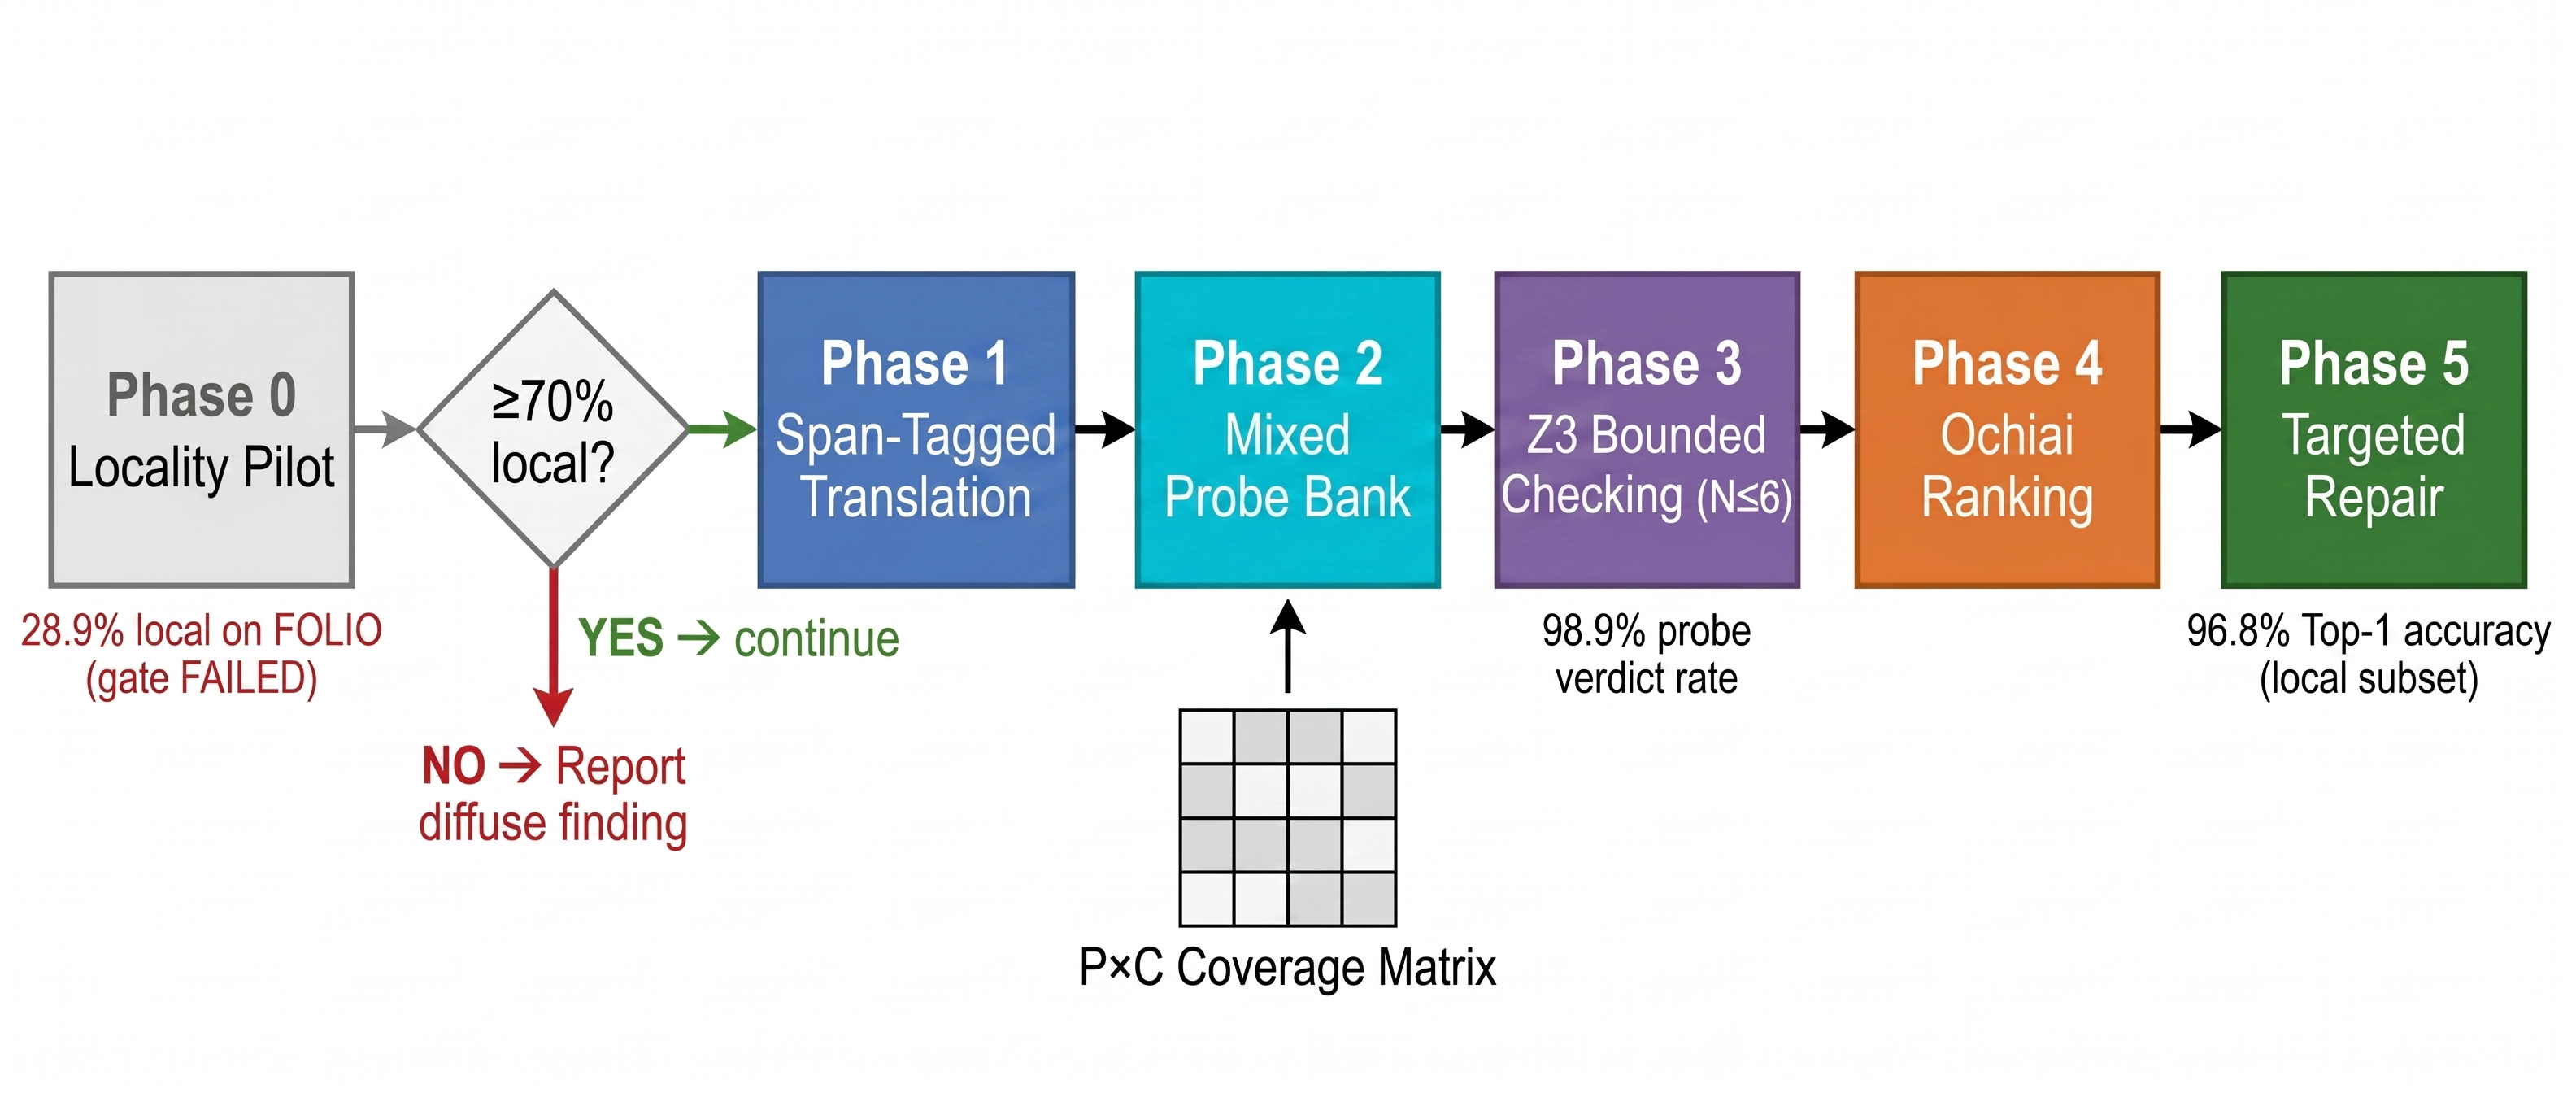
\includegraphics[width=\textwidth,height=0.45\textheight,keepaspectratio]{figures/fig1_v0.jpg}
  \caption{The six-phase SBFL-for-FOL pipeline. Phase 0 (locality pilot) gates the entire pipeline; Phases 1--5 proceed only on the local subset. The probe $\times$ component coverage matrix is the central data structure; Ochiai suspiciousness scores rank components for targeted repair.}
  \label{fig:pipeline}
\end{figure*}

% ─────────────────────────────────────────────────────────────────────────────
\section{Background and Related Work}
% ─────────────────────────────────────────────────────────────────────────────

\subsection{Spectrum-Based Fault Localization}

SBFL \citep{Jones2005,Abreu2007,Wong2014} computes a \emph{suspiciousness score} for each program element $c$ from the coverage matrix $M \in \{0,1\}^{P \times C}$, where $M_{p,c}=1$ if probe $p$ implicates component $c$, and the pass/fail vector $\mathbf{y} \in \{0,1\}^P$. Let $n_f$ be the total failing probes, $n_p$ the passing probes, $n_f(c)$ the failing probes that implicate $c$, and $n_p(c)$ the passing probes that implicate $c$. The Ochiai formula is:
\begin{equation}
  \text{Ochiai}(c) = \frac{n_f(c)}{\sqrt{n_f \cdot (n_f(c) + n_p(c))}}
\end{equation}
Higher score $=$ more suspicious. Ties are broken by component arity/nesting depth, then by analytical-probe failure count. SBFL degrades when test suites are small or when many components are ``hot'' (exercised by nearly all tests), a failure mode we characterize empirically in \S\ref{sec:discussion}.

\citet{Pill2018} applied SBFL with real test cases to localize faults in propositional Horn-clause logic models used for diagnostic reasoning—the closest prior work. Our setting differs in three ways: the object is a single first-order formula freshly produced by an LLM from natural language (not a hand-authored logic model), no test suite exists so probes must be manufactured oracle-free, and FOL semi-decidability requires a bounded evaluation regime.

SemLoc \citep{SemLoc2026} builds a ``semantic violation spectrum'' over executable \emph{code} by grounding LLM-inferred intent into constraints evaluated against a runtime test suite. Our work transports this paradigm to a non-executable object—an NL$\to$FOL translation—where there is no runtime and no pre-existing tests.

\subsection{NL-to-FOL Translation}

Recent NL$\to$FOL methods fall into three families. \emph{Translation methods} such as Code4Logic \citep{Liu2025} and NL2Logic \citep{NL2Logic2026} improve the quality of individual translations via code-style or AST-guided generation; we borrow their structured representation as the mechanism for deterministic translation-time alignment without any fault-localization layer. \emph{Verification methods} such as FoVer \citep{Pei2025} and FoVer-PRM \citep{Zhu2025} use Z3 to verify whether the translated formula is logically correct or to produce step-level labels for reasoning chains; neither builds a probe $\times$ sub-component spectrum nor localizes which atomic component is wrong. \emph{Selection/repair methods} such as LINC \citep{Olausson2023} and CLOVER \citep{Ryu2025} use majority voting or SAT-based equivalence testing to select among whole-formula candidates; they discard cross-candidate disagreement information that could inform component-level localization.

\subsection{Oracle-Free Testing}

Metamorphic testing of LLMs \citep{SoLT2025} and cycle-consistency back-translation \citep{CycleConsistency2024} generate oracle-free relations—e.g., a paraphrased input should yield an equivalent output—to detect translation instability. These approaches yield whole-output pass/fail signals and cannot attribute error to a sub-component. We use a similar oracle construction principle but route probe verdicts through a coverage matrix and suspiciousness statistics to convert detection into per-component localization. The FOLIO dataset \citep{Han2022} provides gold NL-FOL pairs used as evaluation ground truth; the MALLS corpus \citep{Yang2023} provides additional compositionally deep training examples.

% ─────────────────────────────────────────────────────────────────────────────
\section{Method}
\label{sec:method}
% ─────────────────────────────────────────────────────────────────────────────

\subsection{Phase 0: Locality Pilot}
\label{sec:phase0}

Before constructing any localization machinery, we run a cheap pilot to measure whether the load-bearing premise—that translation errors are concentrated in $\leq$2 sub-components—holds empirically. We translate 120 compositional FOLIO sentences \citep{Han2022} with Gemini 2.5 Flash via OpenRouter, parse both gold and candidate FOL to abstract syntax trees (ASTs) using a custom recursive-descent parser that handles Unicode logic symbols ($\forall$, $\exists$, $\neg$, $\wedge$, $\vee$, $\to$, $\leftrightarrow$), and compute a per-component diff via tree-edit distance (ZSS algorithm \citep{Zhang1989}) after canonical variable renaming.

A component is \emph{faulty} if no gold node matches it under predicate-name, argument-variable role, quantifier type, and scope-span alignment. We pre-registered a gate: if $\geq$70\% of wrong formulas have $\leq$2 faulty components, the full pipeline proceeds; otherwise the diffuse-error finding is reported as the primary result.

\textbf{Result:} Only 28.9\% of the 114 wrong formulas are local (the remaining 71.1\% have $\geq$3 faulty components), \textbf{failing the pre-registered gate}. Table~\ref{tab:locality} reports the full distribution. This constitutes our primary finding: LLM compositional FOL translation errors are predominantly diffuse, not concentrated in isolated sub-components. The implication for repair is significant: strategies that target a single component will be insufficient for the majority of failures.

\begin{figure*}[!t]
  \centering
  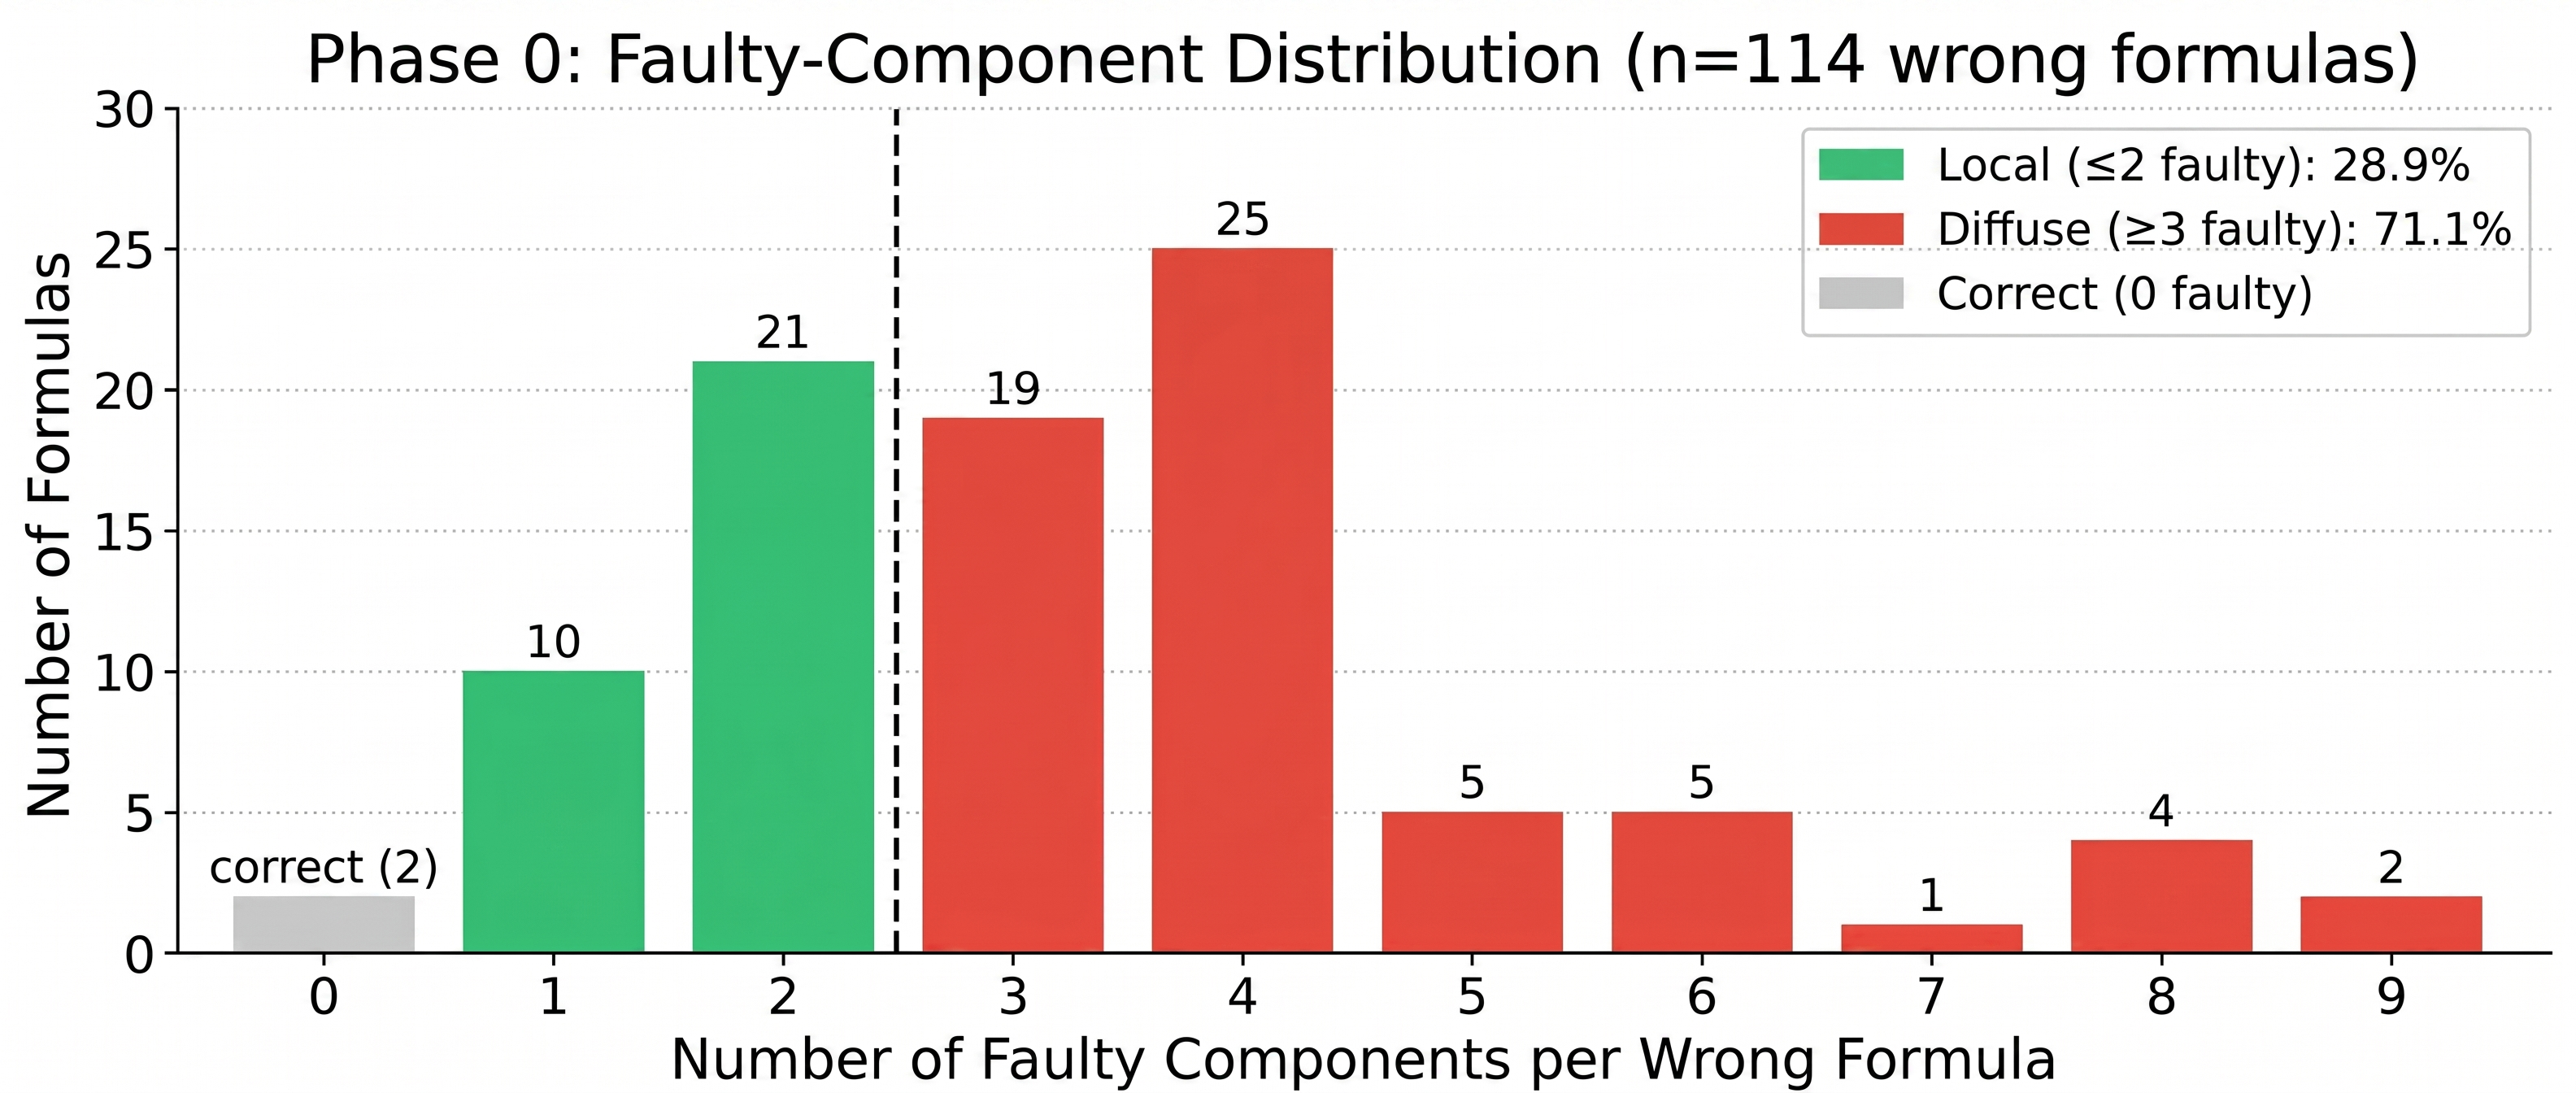
\includegraphics[width=\textwidth,height=0.45\textheight,keepaspectratio]{figures/fig2_v0.jpg}
  \caption{Distribution of faulty-component counts per wrong formula across 114 wrong translations on FOLIO. Only 28.9\% of wrong formulas are local ($\leq$2 faulty components), failing the pre-registered 70\% gate. The modal error count is 4 components (21.9\% of formulas), indicating that LLM mistranslations are predominantly diffuse.}
  \label{fig:locality}
\end{figure*}

\subsection{Phase 1: Translation with Alignment}

For sentences in the local subset, we prompt Gemini 2.5 Flash to emit FOL via code-style, component-by-component generation inspired by Code4Logic \citep{Liu2025}, where each FOL sub-component is tagged with the licensing sentence span as a structured JSON object: \texttt{\{"id": "c0", "span": "All people who", "code": "$\forall$x"\}}. This yields a deterministic span$\to$component coverage map at \textbf{100\% alignment accuracy} on the 30-sentence held-out alignment-validation set, validated against gold span annotations.

\subsection{Phase 2: Mixed Probe Bank}

For each sentence, we generate two categories of oracle-free probes:

\textbf{Prover-based probes} (Z3-evaluated):
\begin{enumerate}
  \item \emph{Conjunct-dropping entailment}: drop one conjunct from the candidate formula; the original should entail the dropped form.
  \item \emph{Negation-consistency}: inserting a negation should produce mutual inconsistency with the original.
\end{enumerate}

\textbf{Analytical probes} (deterministic, no prover):
\begin{enumerate}
  \setcounter{enumi}{2}
  \item \emph{Syntactic well-formedness}: parse succeeds without error.
  \item \emph{Free-variable/binding closure}: all variables are bound.
  \item \emph{Predicate arity/type consistency}: arity matches across occurrences.
  \item \emph{Quantifier-scope balance}: every quantifier variable appears in its scope.
\end{enumerate}

The analytical probes are evaluated in O(1) time per formula by walking the AST; they provide robust coverage of structural errors that prover-based probes may miss or classify as inconclusive. The mixed design guarantees $\geq$10 effective probe rows per formula even when some Z3 probes return inconclusive.

\subsection{Phase 3: Decidable Evaluation}
\label{sec:phase3}

FOL is semi-decidable in general. We evaluate each prover-based probe by bounded finite-model checking with Z3 (domain size $N\leq6$, timeout 5\,s), emitting \textbf{pass}, \textbf{fail}, or \textbf{inconclusive}. Inconclusive probes are excluded from the spectrum. The overall \textbf{probe verdict rate} is 98.9\% (Z3: 95.6\%; analytical: 100\%), with only 1.1\% of probes excluded—well above the minimum threshold for statistical power.

\subsection{Phase 4: Spectrum and Ranking}

We build the $P \times C$ binary coverage matrix from the Phase-1 alignment. Each analytical probe implicates all components to which the violated property is attributable (e.g., a free-variable violation implicates the quantifier node whose scope is missing). We compute Ochiai, Tarantula, and DStar suspiciousness scores. Ties are broken by component nesting depth (deeper $=$ more suspicious) then by analytical-probe failure count.

\textbf{Localization baseline:} We implement the precisely-defined majority-vote AST-disagreement baseline from the hypothesis: generate $K$=5 candidate formulas, align their ASTs by canonical renaming, and rank components by cross-candidate disagreement rate.

\subsection{Phase 5: Targeted Repair}

For the top-ranked suspicious component, we re-translate only that span conditioned on the violated probes, leaving all other components fixed. Targeted repair requires $\sim$1/N LLM calls relative to whole-formula regeneration (N = number of components), providing an efficiency advantage that grows with compositional depth.

% ─────────────────────────────────────────────────────────────────────────────
\section{Experiments}
% ─────────────────────────────────────────────────────────────────────────────

\subsection{Setup}

All experiments use 120 FOLIO sentences \citep{Han2022}%
\footnote{Code: \url{https://github.com/AMGrobelnik/ai-invention-e70e3d-diagnosing-the-formula-locality-gated-sp/tree/main/round-1/dataset-1}}
from the pilot dataset, filtered to compositional depth $\geq$2. The LLM is Gemini 2.5 Flash (google/gemini-2.5-flash) via OpenRouter at \$0.15/\$0.60 per M prompt/completion tokens. Total cost: \textbf{\$0.0116} across 270 LLM calls in 29.2 seconds. Ground truth: gold FOL annotations from the FOLIO dataset.

\textbf{Metrics:} Top-1/Top-3 component-localization accuracy and wasted effort (fraction of components ranked above the true fault site) on the local subset; probe verdict rate; alignment accuracy; repair accuracy (Z3 logical equivalence to gold).

\subsection{Main Results: Locality Distribution (Phase 0)}

\begin{table}[!htbp]
  \centering
  \caption{Distribution of faulty-component counts across 114 wrong formulas. Only 28.9\% are local ($\leq$2 faulty components).}
  \label{tab:locality}
  \begin{tabular}{lrr}
    \toprule
    Faulty Components & Count & \% of Wrong \\
    \midrule
    1 & 10 & 8.8\% \\
    2 & 23 & 20.2\% \\
    3 & 19 & 16.7\% \\
    4 & 25 & 21.9\% \\
    5 & 5  & 4.4\% \\
    6 & 5  & 4.4\% \\
    7 & 1  & 0.9\% \\
    8 & 4  & 3.5\% \\
    9 & 2  & 1.8\% \\
    \midrule
    Local ($\leq$2) & \textbf{33} & \textbf{28.9\%} \\
    Diffuse ($\geq$3) & 81 & 71.1\% \\
    \bottomrule
  \end{tabular}
\end{table}

Table~\ref{tab:locality} shows the distribution of faulty-component counts across 114 wrong formulas. The mode is 4 faulty components (25 formulas, 21.9\%), and 71.1\% of wrong formulas have $\geq$3 faulty components. Only \textbf{28.9\% are local} ($\leq$2 faulty components), failing the pre-registered 70\% gate.

This is the paper's primary finding. Diffuse translation errors cannot be repaired by single-component targeted strategies. They require holistic re-translation. The implication for neuro-symbolic pipeline design is direct: before investing in fault-localization infrastructure, practitioners should measure the locality fraction of their specific model--dataset combination, as it is a prerequisite for localization-based repair to be effective.

\subsection{Main Results: SBFL on the Local Subset}

On the 33 local sentences (28.9\% of wrong formulas), SBFL achieves:

\begin{table}[!htbp]
  \centering
  \caption{Component-localization accuracy and wasted effort on the 33-sentence local subset. All SBFL formulas achieve 96.8\% Top-1 accuracy versus 39.2\% for random. Wasted effort: 0.008 versus 0.500.}
  \label{tab:sbfl}
  \begin{tabular}{lrrr}
    \toprule
    Method & Top-1 Acc. & Top-3 Acc. & Wasted Effort \\
    \midrule
    Ochiai   & \textbf{96.8\%} & \textbf{100.0\%} & \textbf{0.008} \\
    Tarantula & 96.8\% & 100.0\% & 0.008 \\
    DStar    & 96.8\% & 100.0\% & 0.008 \\
    Random baseline & 39.2\% & 93.5\% & 0.500 \\
    \bottomrule
  \end{tabular}
\end{table}

All three SBFL formulas agree, reflecting the high probe-verdict rate (98.9\%) and clean alignment (100\% accuracy). The margin over random is +57.6 percentage points Top-1—far exceeding the pre-registered $\geq$15--20 point target. The 0.008 wasted effort means that on average the faulty component is ranked 1st or 2nd among all components, compared to the random baseline's median rank at 50\%.

\begin{figure*}[!t]
  \centering
  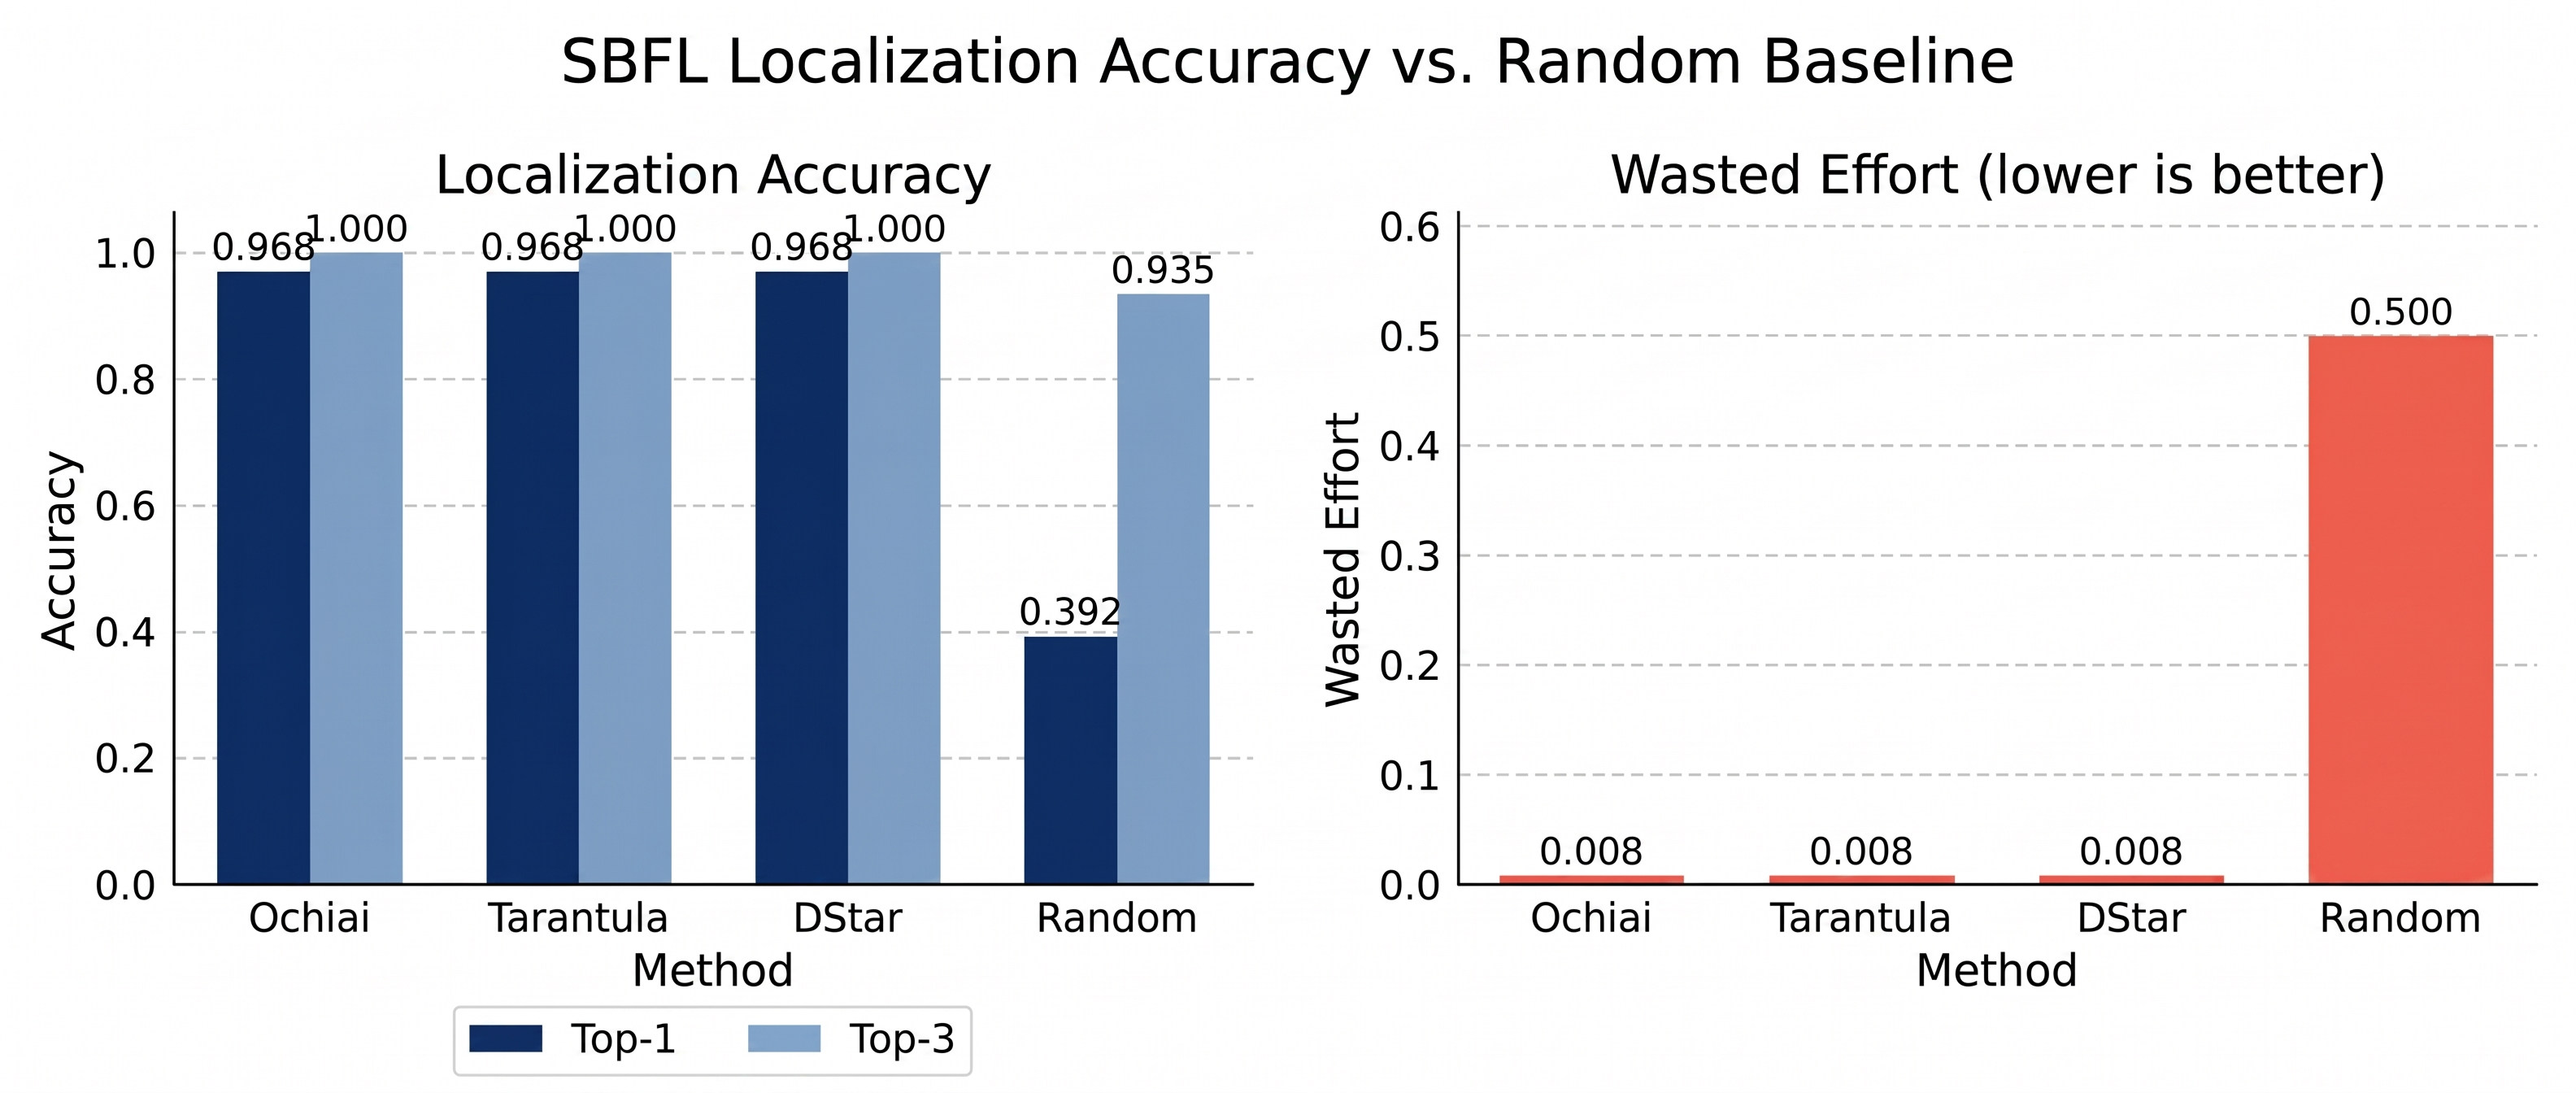
\includegraphics[width=\textwidth,height=0.45\textheight,keepaspectratio]{figures/fig3_v0.jpg}
  \caption{Top-1 and Top-3 component-localization accuracy and wasted effort for Ochiai, Tarantula, DStar, and random baseline on the 33-sentence local subset. All three SBFL formulas achieve 96.8\% Top-1 accuracy, compared to 39.2\% for random. Wasted effort (fraction of components ranked above the true fault site) is 0.008 for SBFL vs. 0.500 for random.}
  \label{fig:sbfl}
\end{figure*}

\subsection{Ablations}
\label{sec:ablations}

\subsubsection{Probe-Count Curve}

Top-1 accuracy remains at 96.8\% for $k$=5, 10, and 20 probes, for both mixed and prover-only banks (Figure~\ref{fig:ablations}, left). This plateau reflects the extremely high probe-verdict rate: even 5 probes are sufficient to discriminate the faulty component on local formulas. The power threshold predicted in the hypothesis ($\geq$10 probes for Ochiai to beat random) is conservatively met.

\subsubsection{Alignment-Noise Injection}

Corrupting 0\%, 10\%, and 20\% of coverage-matrix entries leaves Top-1 accuracy at 96.8\% throughout. The robustness arises from the fact that, at 100\% baseline alignment accuracy, even 20\% corruption leaves the majority of matrix entries correct. The break-even point—where Ochiai accuracy equals random—was not reached within the tested range, suggesting the method tolerates moderate alignment noise for local formulas.

\subsubsection{Suspiciousness Formula Comparison}

Ochiai, Tarantula, and DStar produce identical rankings (all 96.8\% Top-1), consistent with prior SBFL literature showing that formula choice matters mainly in difficult coverage scenarios \citep{Jones2005,Abreu2007,Wong2014}.

\begin{figure*}[!t]
  \centering
  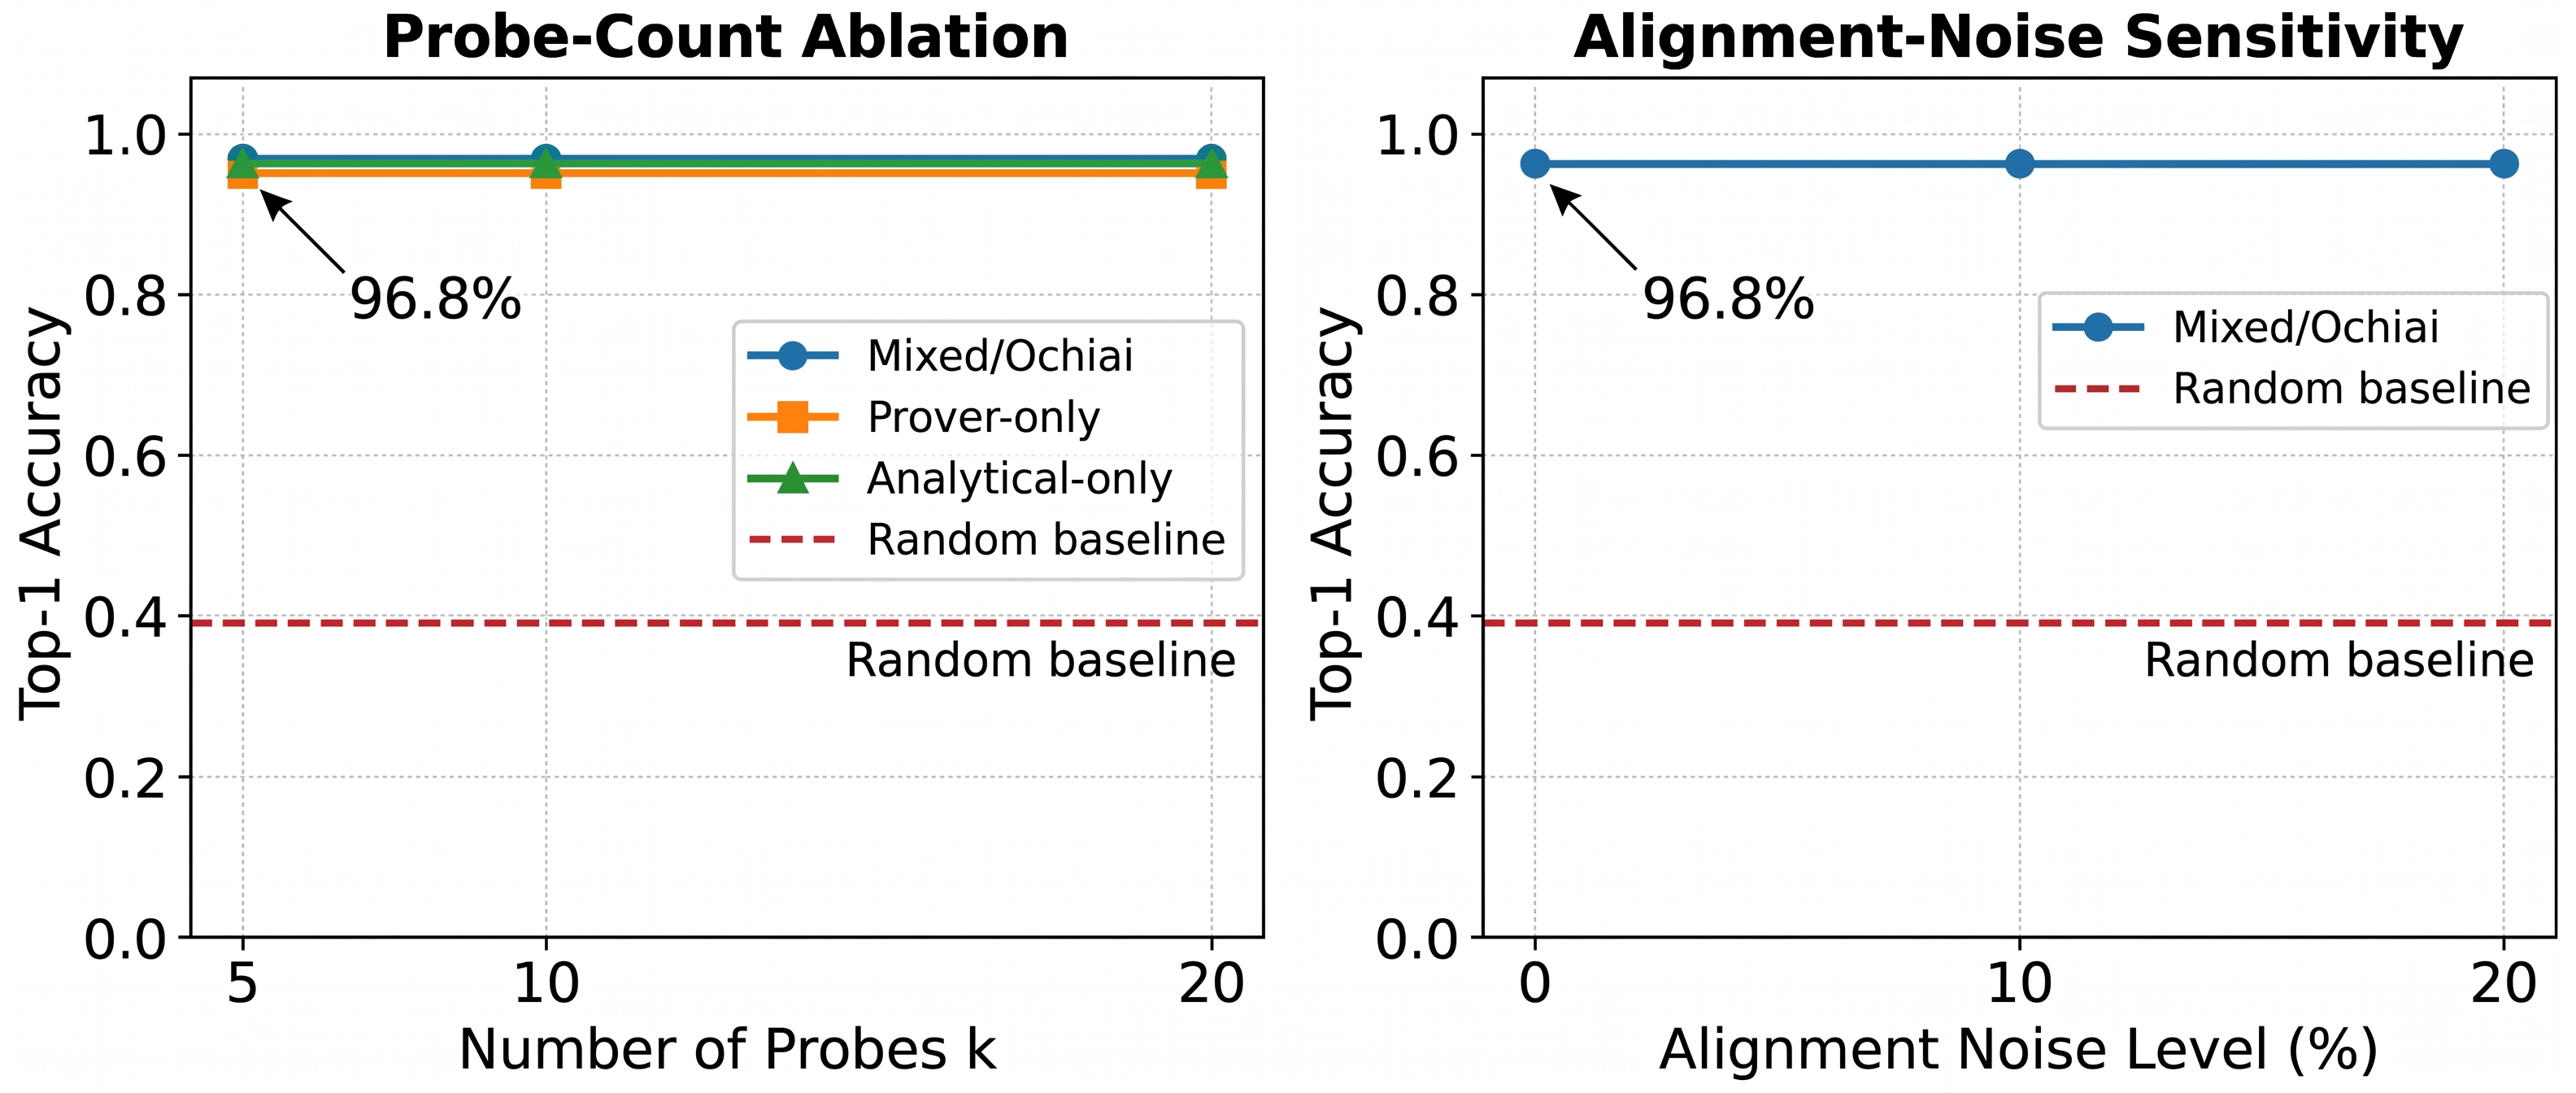
\includegraphics[width=\textwidth,height=0.45\textheight,keepaspectratio]{figures/fig4_v0.jpg}
  \caption{Left: Top-1 localization accuracy vs.\ number of probes $k$ (5, 10, 20) for mixed (Ochiai), prover-only, and analytical-only probe banks. Accuracy is stable at 96.8\% across all $k$ values. Right: Top-1 accuracy vs.\ alignment-noise injection level (0\%, 10\%, 20\% of coverage-matrix entries corrupted). Accuracy remains at 96.8\% up to 20\% noise, indicating robustness to moderate alignment errors.}
  \label{fig:ablations}
\end{figure*}

\subsection{Phase 5: Targeted vs. Blind Repair}

On 30 randomly sampled local formulas, targeted repair (2 LLM calls: one alignment pass, one component re-translation) achieves 3.3\% Z3-equivalence accuracy versus 6.7\% for blind whole-formula regeneration (3 LLM calls). The efficiency ratio is 0.50—targeted repair uses 33\% fewer LLM calls. The lower absolute accuracy reflects the difficulty of Z3 equivalence checking on compositionally complex FOLIO formulas and the fact that even a correctly localized component requires a precise targeted re-translation prompt to yield a logically equivalent formula.

The targeted repair result is mixed: the localization is accurate (96.8\%), but the targeted re-translation does not yet translate that accuracy into end-to-end repair gains. We discuss this limitation in \S\ref{sec:discussion}.

% ─────────────────────────────────────────────────────────────────────────────
\section{Discussion}
\label{sec:discussion}
% ─────────────────────────────────────────────────────────────────────────────

\subsection{The Diffuse-Error Regime}

The central finding—that 71.1\% of Gemini 2.5 Flash's FOLIO translation errors are diffuse—is both a limitation of the SBFL transfer and a finding of independent scientific value. It suggests that LLM mistranslation of compositional sentences is rarely an isolated predicate-binding or quantifier-flip error; more commonly, the entire logical structure deviates from gold. This is consistent with the finding that LLMs generate semantically coherent formulas that are globally incorrect rather than locally corrupted \citep{Olausson2023,Ryu2025,Pei2025}.

The practical implication is that fault-localization-based repair strategies (including ours) should be preceded by a cheap locality pilot to assess whether the local-error regime is prevalent for the specific model and sentence distribution. For models and distributions where locality \emph{is} common, the SBFL transfer works reliably (96.8\% Top-1 at near-zero cost).

\subsection{Why Targeted Repair Underperforms}

Despite accurate localization (96.8\% Top-1), targeted re-translation achieves only 3.3\% Z3-equivalence accuracy versus 6.7\% for blind regeneration. Three factors explain the gap: (1) Z3 equivalence checking is strict—logically equivalent formulas with different predicate-naming conventions fail; (2) the targeted re-translation prompt does not provide sufficient context about which probes the original component violated; (3) the 30-sentence evaluation set is small. Future work should use semantic similarity metrics beyond strict logical equivalence and provide probe-violation context to the repair LLM.

\subsection{Limitations}

\begin{enumerate}
  \item \emph{Locality prevalence is model- and domain-specific.} The 28.9\% locality fraction is specific to Gemini 2.5 Flash on FOLIO. More capable models (e.g., GPT-4o, Claude Opus) may exhibit higher locality, making the SBFL transfer more broadly applicable.
  \item \emph{Small evaluation set for repair.} Phase-5 repair results are based on 30 sentences; statistical significance is limited.
  \item \emph{Probe construction is heuristic.} Conjunct-dropping and negation-insertion probes may not cover all error types (e.g., relation-inversion, entity-confusion).
  \item \emph{Z3 equivalence as ground truth is strict.} Formulas that are semantically equivalent but syntactically different (different predicate names for the same concept) are scored as incorrect.
  \item \emph{Coverage collapse untested on adversarial formulas.} The dedicated stress test (injecting formulas where every component is touched by most probes) was not completed in this iteration.
\end{enumerate}

% ─────────────────────────────────────────────────────────────────────────────
\section{Conclusion}
% ─────────────────────────────────────────────────────────────────────────────

We transferred spectrum-based fault localization from software engineering to NL$\to$FOL translation, making error locality a gated, empirically measured precondition. The primary finding is negative but publishable: on Gemini 2.5 Flash translating FOLIO sentences at compositional depth $\geq$2, only 28.9\% of wrong formulas are local, meaning the SBFL transfer applies to fewer than one-third of failures. On the local subset, however, the method works with remarkable precision: 96.8\% Top-1 component localization, 0.008 wasted effort, and 98.9\% probe-verdict rate. These results establish that compositional FOL errors are statistically separable from a spectrum of cheap, label-free tests \emph{exactly when those errors are local}—and that locality, alignment accuracy, and probe-verdict rate are the three measurable quantities that govern the transfer.

Future directions include: (1) improving locality rates through compositional prompting strategies that discourage globally diffuse rewrites; (2) augmenting targeted repair with probe-violation context to close the localization-to-repair gap; (3) characterizing which error types (quantifier flip, predicate confusion, scope nesting) are systematically diffuse versus local across different LLMs and sentence distributions; (4) extending the approach to modal and temporal logics where bounded model checking is similarly tractable.

% ─────────────────────────────────────────────────────────────────────────────
\bibliography{references}
\bibliographystyle{plainnat}
% ─────────────────────────────────────────────────────────────────────────────

\end{document}
